
\subsection{Network Interpretability}

\noindent To try and understand why the network was classifying as it was, we decided to look at the node values of the penultimate layer of the trained network. This dense layer of 1024 nodes feeds into the final dense layer with 3 nodes, one for each of the classification types. By looking at the node activation layer, patterns emerge as to the importance of each node, and how the model has trained the weights and biases to learn how to classify each image for the result to be produced in the final output layer.\medskip

\begin{figure}[t!]
 \centering
 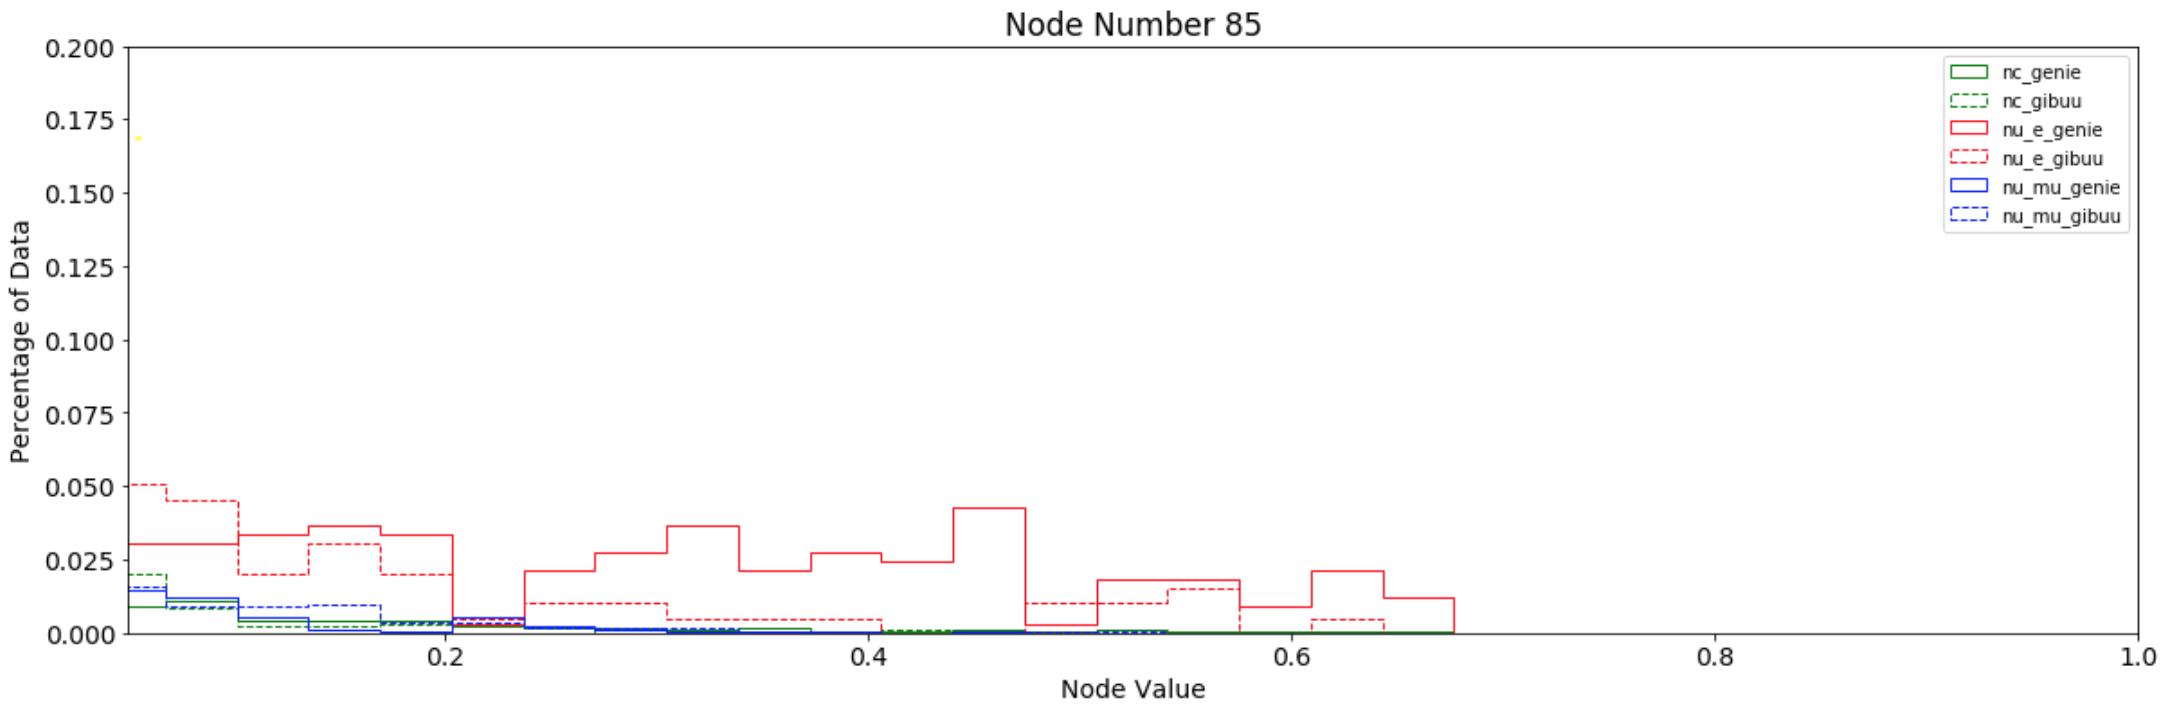
\includegraphics[width=160mm]{nodes/node01.png}
 
 \textbf{Figure 28.} \textit{Node activation values, for Node 85, for events of all three types and both event generators from the training process in section 3.1.4, where the network was trained and tested on equal GENIE and GiBUU combined data over 100 epochs.}

 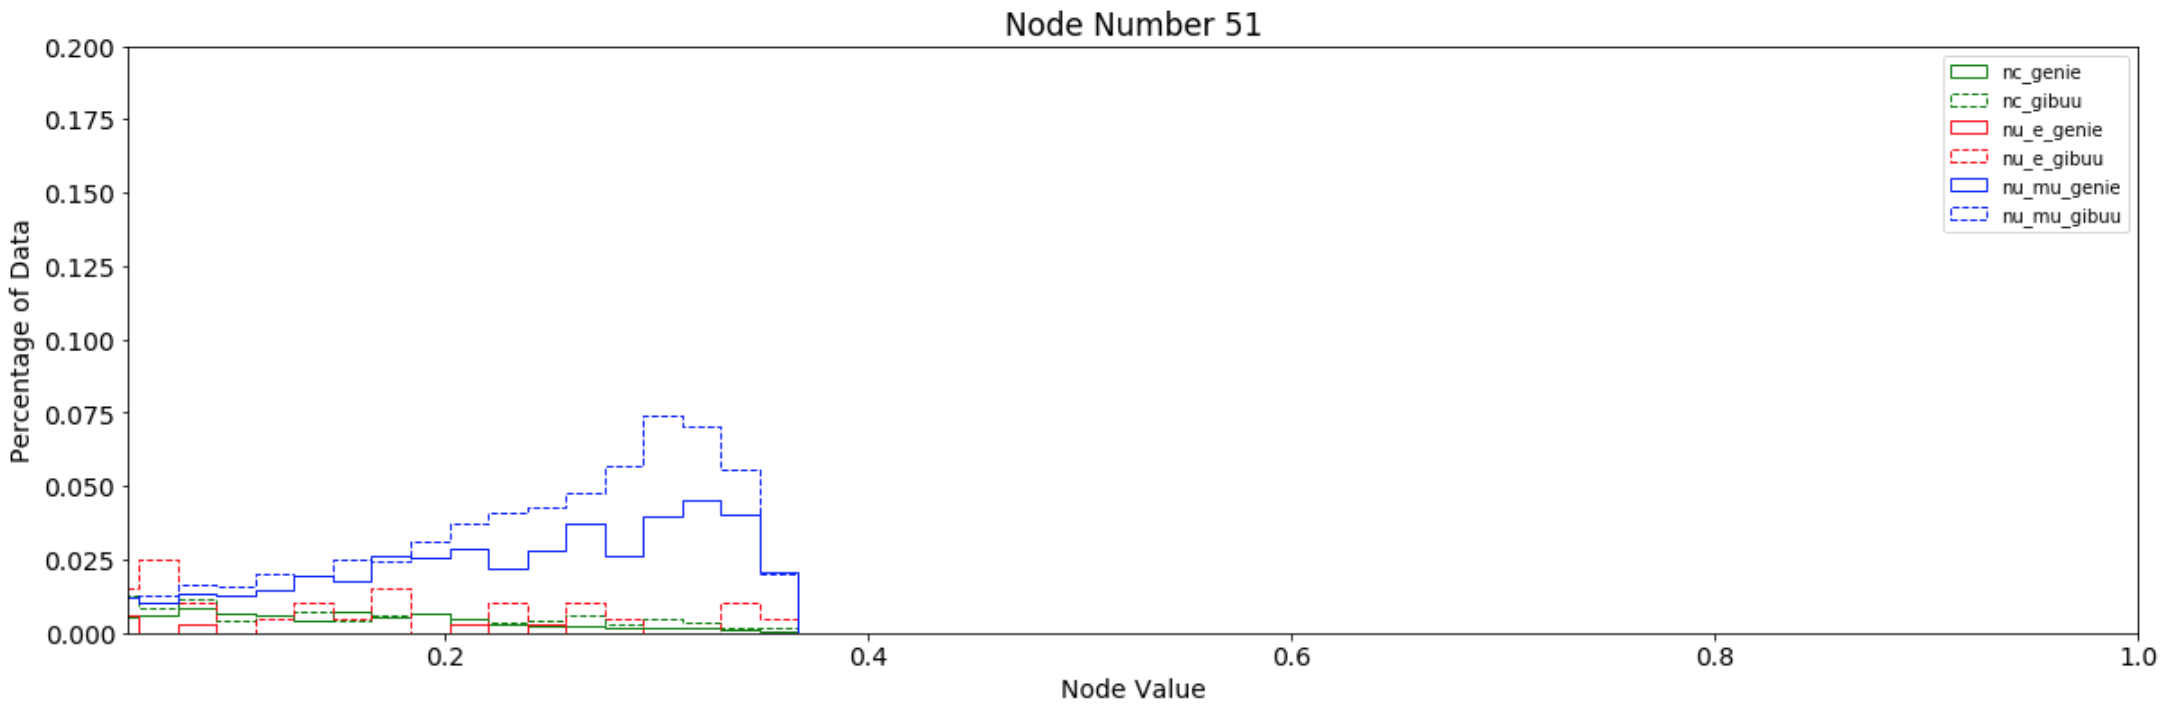
\includegraphics[width=160mm]{nodes/node02.png}
 
 \textbf{Figure 29.} \textit{Node activation values, for Node 51, for events of all three types and both event generators from the training process in section 3.1.4.}

 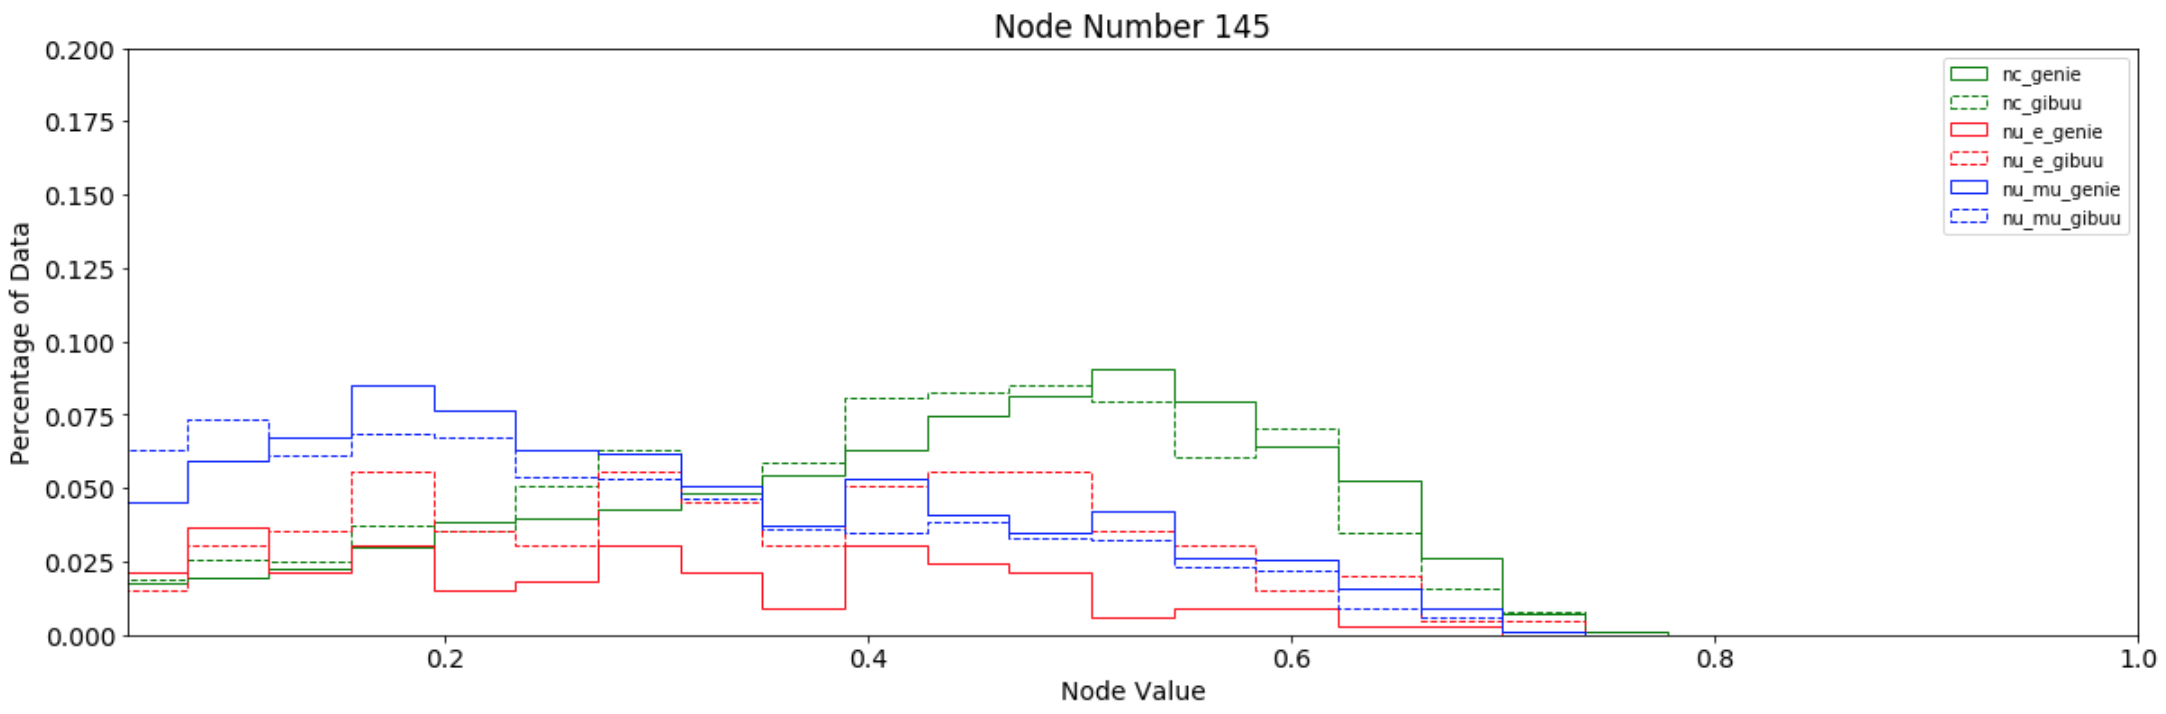
\includegraphics[width=160mm]{nodes/node03.png}
 
 \textbf{Figure 30.} \textit{Node activation values, for Node 145, for events of all three types and both event generators from the training process in section 3.1.4.}
\end{figure}



\noindent This analysis was performed on the classifier trained in section 3.1.4, which contained an equal number of events of each of the interaction type and from GENIE and GiBUU. The majority of the nodes in the final layer, 78.4\%, did not activate for any of the events and as a result would have no impact on the final classification. By plotting a histogram of the values of the nodes, and separating the distributions depending on interaction type and generator source, it became clear that activation of certain nodes indicates how the model will classify the event. An example was node 85, see Figure 28, here it can be seen that, on the most part, if the node is activated, the event will be classified as a $\nu_e$ event, especially at large values. This is also visible in Figure 29, where activation mostly indicates that the event will be classified as a $\nu_\mu$ event, and this is more apparent at large values of the node.\medskip

\noindent With some nodes, see Figure 20, certain values of the node indicate the classification of the event, with overlapping regions of the distributions visible. While many indicate the domain source of the event. This can be seen in Figure 31, where the largest values of the node activation are produced when the event is a GiBUU produced $\nu_\mu$ event. In Figure 32, the largest activation values occur when a GENIE produced $\nu_e$ event is passed through the network for classification.\medskip

\begin{figure}[t!]
 \centering
 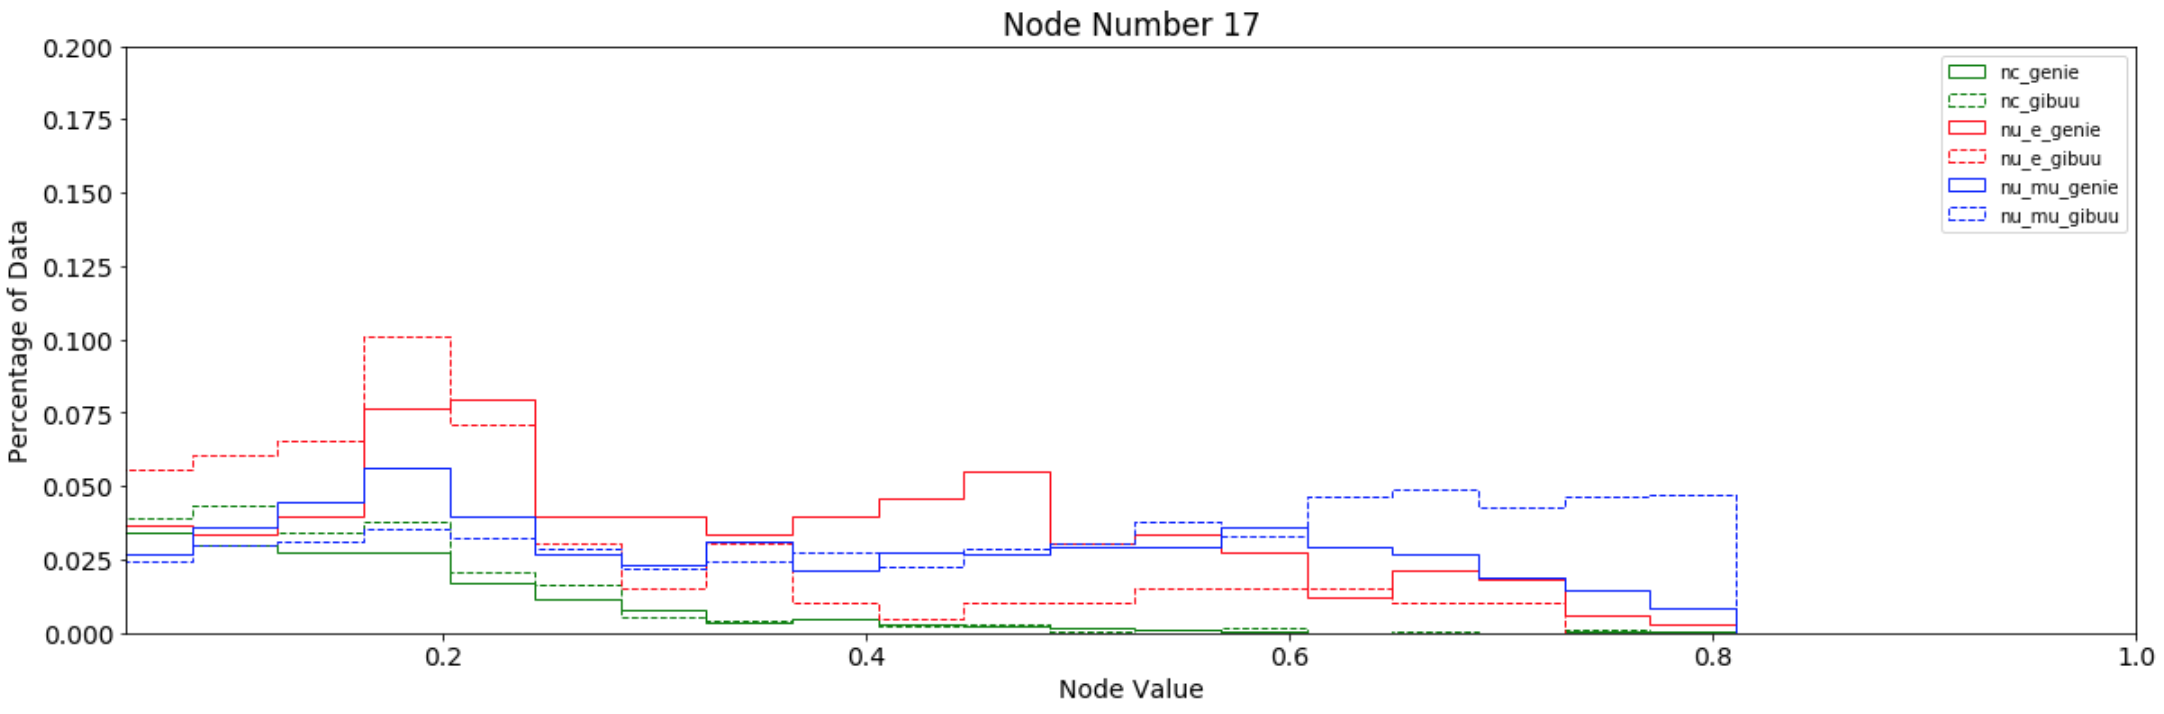
\includegraphics[width=160mm]{nodes/node04.png}
 
 \textbf{Figure 31.} \textit{Node activation values, for Node 17, for events of all three types and both event generators from the training process in section 3.1.4.}

 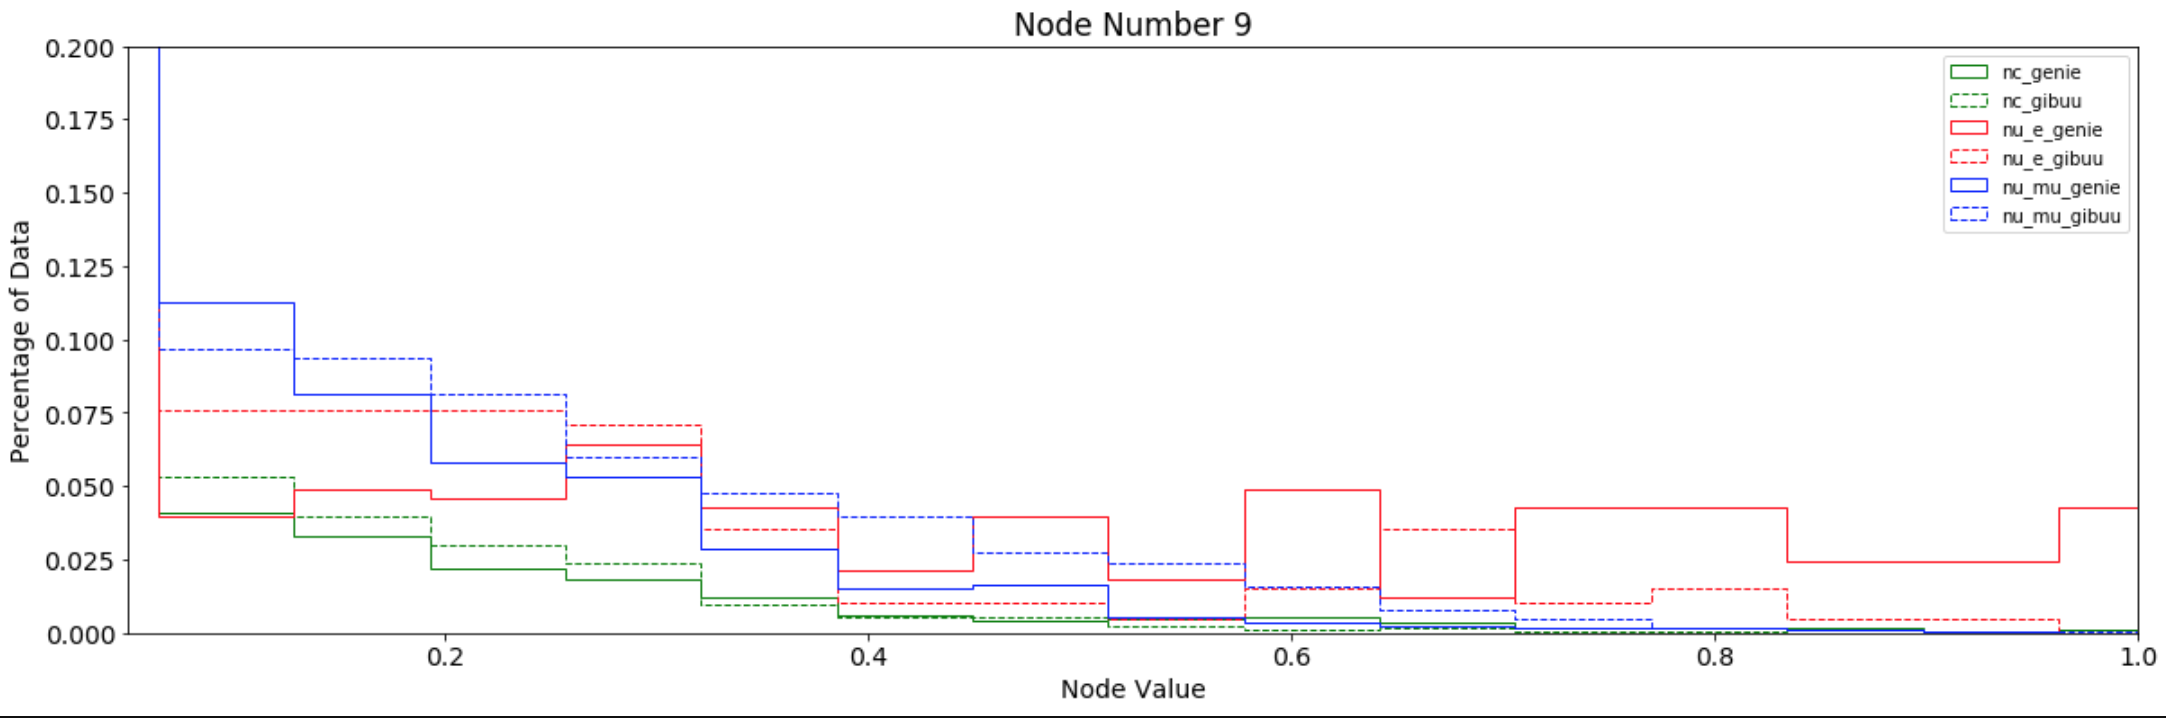
\includegraphics[width=160mm]{nodes/node05.png}
 
 \textbf{Figure 32.} \textit{Node activation values, for Node 9, for events of all three types and both event generators from the training process in section 3.1.4.}
\end{figure}

\noindent In order to be able to determine any patterns over the entirety of the penultimate node layer, rather than using qualitative methods on an individual basis, the node activation values were treated as distributions, for the various event types. Here the event types consisted of the 3 event interaction types and the two event generators. The maximum value of the purity efficiency functions was taken to represent each interaction type for each node. For each interaction type, ie. GENIE generated or $\nu_\mu$, an array was produced for the maximum purity efficiency values for each node. In order to see if there were any correlations between the values for each interaction type the arrays were plotted against each other as scatter plots.\medskip

\noindent While this may not be the most robust operation, what it does enable it the quantification of the separation of these node value distributions. By treating the node histograms as distributions, a purity efficiency curve will determine the separation of that distribution, from the background- the other event types. As significant patterns are being looked for in the higher values of nodes, as these are where greater activation has taken place, a purity efficiency calculation is appropriate, as these methods are used for classifications where correct classification is given by greater activation at higher confidence levels.\medskip

\begin{figure}[h]
 \centering
 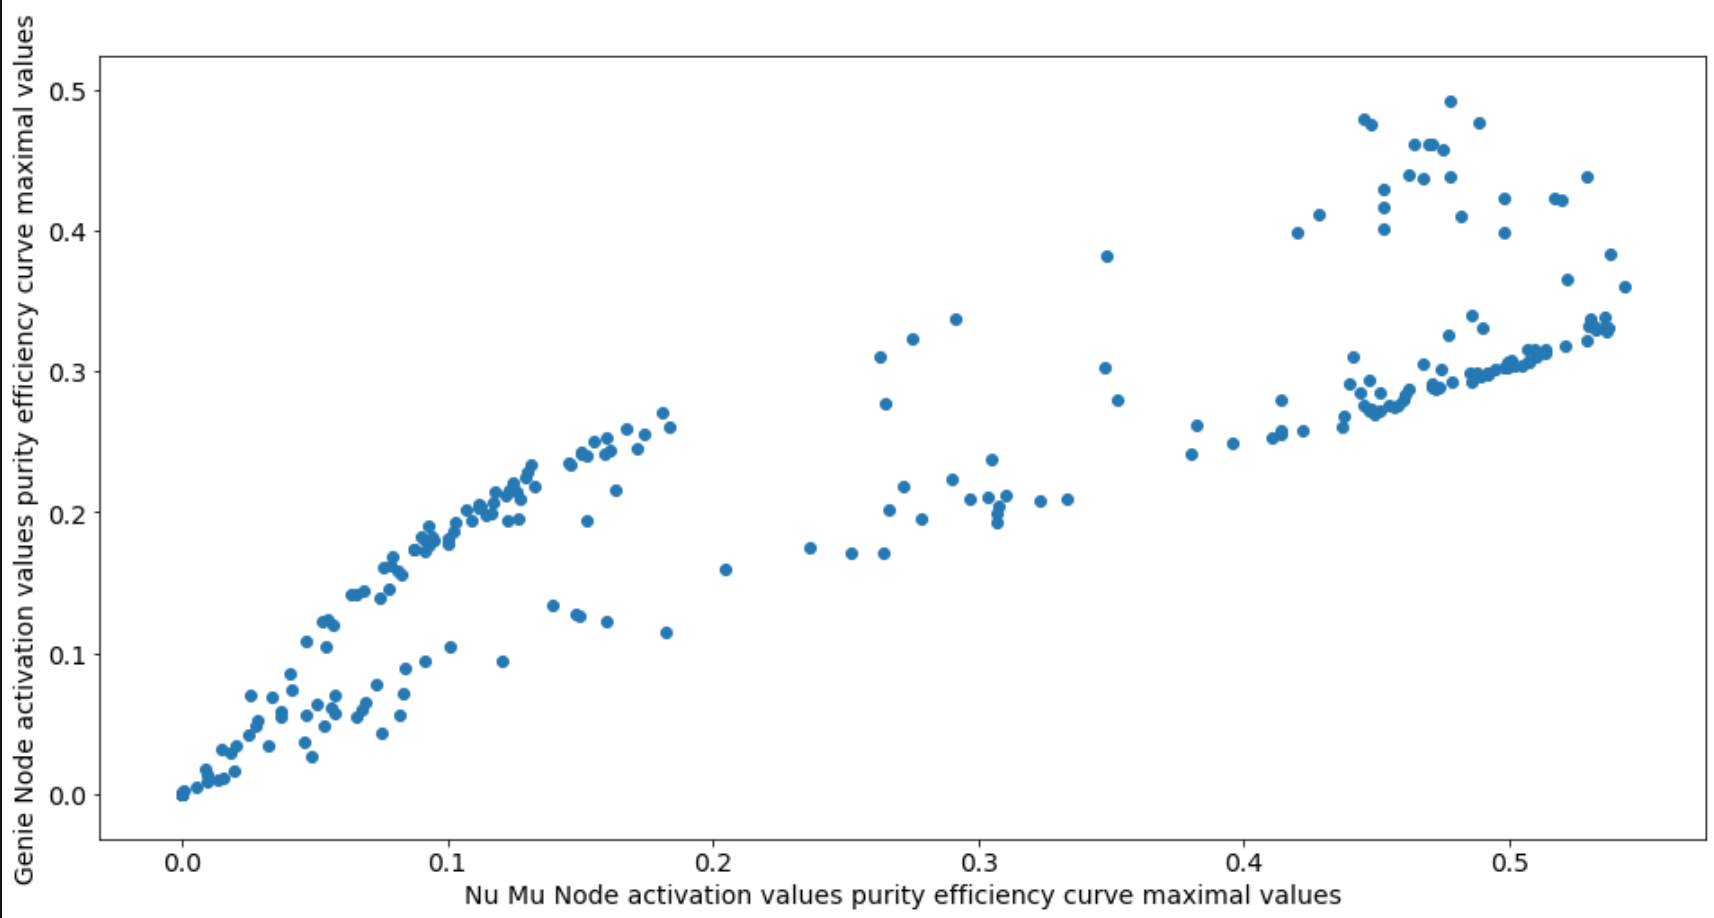
\includegraphics[width=100mm]{nodes/nodes2.png}
 
 \textbf{Figure 33.} \textit{Node activation values purity efficiency curve maximal values over all nodes to see the correlation between $\nu_\mu$ events and GibUU generated events}

\end{figure}

\noindent Most combinations showed no correlation, however the strongest correlation can be seen between the $\nu_\mu$ events and the GibUU events. This indicates that node activation where there was a measured separation were able to measure such for certain nodes for both $\nu_\mu$ events and GibUU events. An example of this would be Figure 33, where the largest activation was seen by GibUU produced $\nu_\mu$ event. The strong positive correlation indicates that there is a correlation between how easily the classifier classified the event, and if that event was a $\nu_\mu$ produced by GibUU produced, meaning these events have features that make them easily identifiable, or have features that were well learned by the model.\medskip



